\section{Runtime Representation of Matches}

To implement matches, two classes are defined - \texttt{Match} and \texttt{Binding}, as seen in Figure \ref{class-diagram-match-binding}.

\begin{figure}[H]
	\centering
	\makebox[\textwidth][c] { 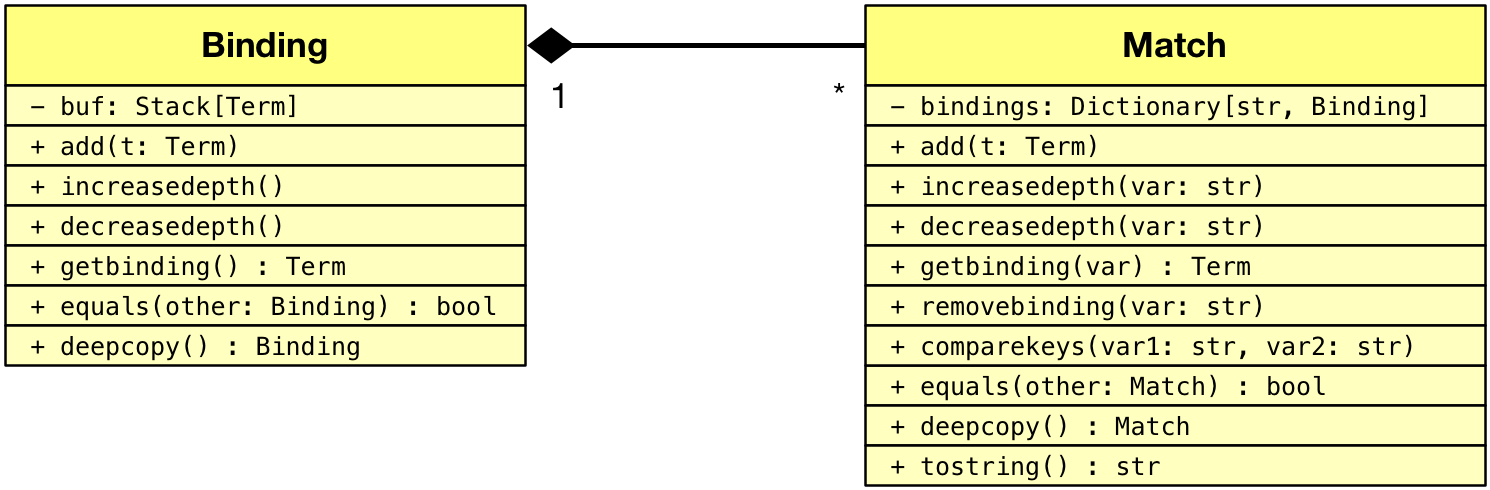
\includegraphics[scale=0.25]{class-diagram-match-binding.png} }
	\caption{Representation of matches.}
\label{class-diagram-match-binding}
\end{figure}

\texttt{Binding} class encapsulates a stack of terms and provides three methods for its manipulation:

\begin{itemize}
\item 
\texttt{increase\_depth} pushes term \texttt{Sequence} onto the stack provided a term on top of the stack is also a \texttt{Sequence}, otherwise raises an error.

\item
\texttt{decrease\_depth} has the following behaviour:
	\begin{enumerate}
		\item
        if stack is empty, raise exception
		\item
		if stack size is 1 and topmost element is not term \texttt{Sequence} raise exception.
		\item
		if stack size is 1 and topmost element is term \texttt{Sequence} do nothing.
		\item
        if stack size > 1, pop topmost element and append it to element below. ( works because increasedepth must be called beforehand)
	\end{enumerate}

\item
\texttt{add(term)} has the following behaviour:
	\begin{enumerate}
		\item
         if stack is empty, add value
		\item
         if stack is not empty and not a compoundarray, raise exception
		\item
        if stack is not empty and is compoundarray, add value to the array.
		\item
        if stack size > 1, pop topmost element and append it to element below. ( works because increasedepth must be called beforehand)
	\end{enumerate}

\item
\texttt{add(term)} has the following behaviour:
	\begin{enumerate}
		\item
         if stack is empty, add value
		\item
         if stack is not empty and not a compoundarray, raise exception
		\item
        if stack is not empty and is compoundarray, add value to the array.
	\end{enumerate}
\end{itemize}



\texttt{Match} class associates pattern-variable with \texttt{Binding} instance.

\begin{itemize}
\item
\texttt{increase\_depth} calls \texttt{increase\_depth} method of relevant \texttt{Binding} instance.

\item
\texttt{decrease\_depth} calls \texttt{decrease\_depth} method of relevant \texttt{Binding} instance.

\item
\texttt{addtobinding} calls \texttt{add} method of relevant \texttt{Binding} instance with \texttt{term}.

\item
\texttt{comparekeys(key1, key2)} compares topmost terms on stacks of bindings assigned to key1 and key2.

\item
	\texttt{deepcopy} creates a new Match instance with all \texttt{Binding} and \texttt{Term} instances contained within copied using \texttt{deepcopy}.
\end{itemize}
